
	\tikzset{every picture/.style={line width=0.75pt}} %set default line width to 0.75pt        
	
	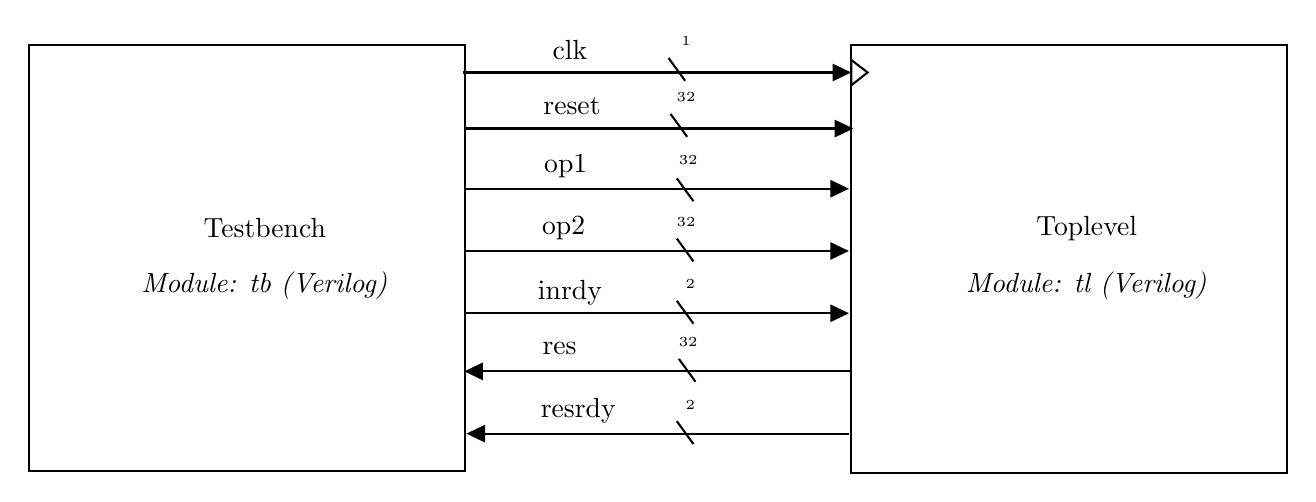
\begin{tikzpicture}[x=0.75pt,y=0.75pt,yscale=-1,xscale=1]
	%uncomment if require: \path (0,406); %set diagram left start at 0, and has height of 406
	
	%Shape: Rectangle [id:dp9211023518838333] 
	\draw   (28.25,60.54) -- (238.5,60.54) -- (238.5,266) -- (28.25,266) -- cycle ;
	%Straight Lines [id:da9591337699307748] 
	\draw    (239.17,130) -- (420.4,130) ;
	\draw [shift={(423.4,130)}, rotate = 180] [fill={rgb, 255:red, 0; green, 0; blue, 0 }  ][line width=0.08]  [draw opacity=0] (8.93,-4.29) -- (0,0) -- (8.93,4.29) -- cycle    ;
	
	%Straight Lines [id:da579702478769955] 
	\draw    (239.17,160) -- (420.4,160) ;
	\draw [shift={(423.4,160)}, rotate = 180] [fill={rgb, 255:red, 0; green, 0; blue, 0 }  ][line width=0.08]  [draw opacity=0] (8.93,-4.29) -- (0,0) -- (8.93,4.29) -- cycle    ;
	
	%Straight Lines [id:da76113659482319] 
	\draw    (239.17,190) -- (420.4,190) ;
	\draw [shift={(423.4,190)}, rotate = 180] [fill={rgb, 255:red, 0; green, 0; blue, 0 }  ][line width=0.08]  [draw opacity=0] (8.93,-4.29) -- (0,0) -- (8.93,4.29) -- cycle    ;
	
	%Straight Lines [id:da45600723803220433] 
	\draw    (238.5,101) -- (422.5,101) ;
	\draw [shift={(425.5,101)}, rotate = 180] [fill={rgb, 255:red, 0; green, 0; blue, 0 }  ][line width=0.08]  [draw opacity=0] (8.93,-4.29) -- (0,0) -- (8.93,4.29) -- cycle    ;
	
	%Shape: Triangle [id:dp124533916535147] 
	\draw   (432.43,73.96) -- (424.51,67.94) -- (424.63,80.14) -- cycle ;
	%Straight Lines [id:da1421875224201805] 
	\draw    (340.5,125) -- (348.5,136) ;
	
	
	%Straight Lines [id:da13538438410660247] 
	\draw    (340.5,154) -- (348.5,165) ;
	
	
	%Straight Lines [id:da5317963116700639] 
	\draw    (340.5,184) -- (348.5,195) ;
	
	
	%Straight Lines [id:da8132393230886649] 
	\draw    (337.5,94) -- (345.5,105) ;
	
	
	%Shape: Rectangle [id:dp6892399379315668] 
	\draw   (424.25,60.54) -- (634.5,60.54) -- (634.5,267) -- (424.25,267) -- cycle ;
	%Straight Lines [id:da04738946392112342] 
	\draw    (241.14,218) -- (424.5,218) ;
	
	\draw [shift={(238.14,218)}, rotate = 0] [fill={rgb, 255:red, 0; green, 0; blue, 0 }  ][line width=0.08]  [draw opacity=0] (8.93,-4.29) -- (0,0) -- (8.93,4.29) -- cycle    ;
	%Straight Lines [id:da32617397066684783] 
	\draw    (341.5,212) -- (349.5,223) ;
	
	
	%Straight Lines [id:da8691621982326109] 
	\draw    (242.17,248) -- (423.4,248) ;
	
	\draw [shift={(239.17,248)}, rotate = 0] [fill={rgb, 255:red, 0; green, 0; blue, 0 }  ][line width=0.08]  [draw opacity=0] (8.93,-4.29) -- (0,0) -- (8.93,4.29) -- cycle    ;
	%Straight Lines [id:da7911020252616261] 
	\draw    (340.5,242) -- (348.5,253) ;
	
	
	%Straight Lines [id:da25458565339624795] 
	\draw    (237.5,74) -- (421.5,74) ;
	\draw [shift={(424.5,74)}, rotate = 180] [fill={rgb, 255:red, 0; green, 0; blue, 0 }  ][line width=0.08]  [draw opacity=0] (8.93,-4.29) -- (0,0) -- (8.93,4.29) -- cycle    ;
	
	%Straight Lines [id:da27828416860185] 
	\draw    (336.5,67) -- (344.5,78) ;
	
	
	
	% Text Node
	\draw (142,149) node   [align=left] {Testbench};
	% Text Node
	\draw (287,119) node   [align=left] {op1};
	% Text Node
	\draw (286,149) node   [align=left] {op2};
	% Text Node
	\draw (289,180) node   [align=left] {inrdy};
	% Text Node
	\draw (290,90) node   [align=left] {reset};
	% Text Node
	\draw (347,176) node   [align=left] {{\tiny 2}};
	% Text Node
	\draw (345,146) node   [align=left] {{\tiny 32}};
	% Text Node
	\draw (346,116) node   [align=left] {{\tiny 32}};
	% Text Node
	\draw (142,183) node   [align=left] {\textit{Module: tb (Verilog)}\\};
	% Text Node
	\draw (538,149) node   [align=left] {Toplevel};
	% Text Node
	\draw (538,183) node   [align=left] {\textit{Module: tl (Verilog)}\\};
	% Text Node
	\draw (284,207) node   [align=left] {res};
	% Text Node
	\draw (346,204) node   [align=left] {{\tiny 32}};
	% Text Node
	\draw (293,237) node   [align=left] {resrdy};
	% Text Node
	\draw (347,234) node   [align=left] {{\tiny 2}};
	% Text Node
	\draw (289,63) node   [align=left] {clk};
	% Text Node
	\draw (345,59) node   [align=left] {{\tiny 1}};
	% Text Node
	\draw (345,86) node   [align=left] {{\tiny 32}};
	
	
	\end{tikzpicture}
	